\documentclass[12pt, letterpaper]{article}
\usepackage[margin=1in]{geometry}
\usepackage{mathptmx}
\usepackage{amsmath}
\usepackage{graphicx}
\usepackage{booktabs}
\usepackage[font={small,it}, justification=centering, labelfont=bf]{caption}
\usepackage{float}
\usepackage[skip=4pt]{parskip}
\usepackage{hyperref}
\hypersetup{colorlinks=true, linkcolor=blue, urlcolor=blue}
\usepackage{listings}
\usepackage{xcolor}
\usepackage{needspace}
\usepackage{titlesec}
\titlespacing*{\section}{0pt}{8pt}{4pt}
\titlespacing*{\subsection}{0pt}{6pt}{2pt}
\renewcommand{\thesection}{\Roman{section}}
\titleformat{\section}{\normalfont\bfseries\large}{\thesection.}{0.5em}{}
\renewcommand{\thesubsection}{\arabic{subsection}}
\titleformat{\subsection}{\normalfont\bfseries}{\thesubsection.}{0.5em}{}

\lstset{
  basicstyle=\ttfamily\small,
  keywordstyle=\color{blue!70!black},
  commentstyle=\color{gray!60},
  columns=fullflexible,
  keepspaces=true,
  frame=single,
  breaklines=true
}

\begin{document}

\begin{center}
  {\Large \textbf{CDA 3201L Lab \#9 Deliverable}}\\[10pt]
  {\large \textbf{Field Programmable Logic Devices (FPGA)}}\\[20pt]
  \begin{tabular}{ll}
    \textbf{Name:} Tuan Khang Phan & \textbf{UID:} U30382645 \\[4pt]
    \textbf{Name:} Huu Phat Nguyen & \textbf{UID:} U46082380 \\
  \end{tabular}
\end{center}

\noindent
This document answers Lab~9 questions 1--4 from \texttt{CDA3201L-Fall23-Lab-9.pdf}.  The
handout states that the deliverable is these answers (with work shown); we typeset them for
clarity and include the requested schematic capture where indicated.

% ─────────────────────────────────────────────
\section{Introduction}

The lab introduces Xilinx FPGAs using Vivado.  We targeted part \texttt{xc7s25csga225-1}
(Spartan-7), created RTL project files \texttt{counter.v} and constraints \texttt{const.xdc},
ran synthesis, implementation, and bitstream generation, and programmed the board so four LEDs
display \texttt{count[3:0]} in binary with a pushbutton reset.

% ─────────────────────────────────────────────
\section{Lab Assignment --- Questions and Answers}

\subsection{(5 pts) How does an FPGA work?  What circuits can it implement?}

\textbf{Answer (own words).}  An FPGA is a chip full of many small, identical configurable
blocks (CLBs) wired together through programmable routing.  Each block can implement a
combinational truth table in lookup tables (LUTs) and usually includes a flip-flop so both
logic and state can be built.  The ``program'' is a \emph{bitstream}: when loaded, it sets
the LUT contents and the switch matrix that connects block outputs to inputs.

Because any Boolean function can be written as sums of products (and sequential systems add
registers and feedback), an FPGA can implement essentially \textbf{any digital circuit} that
fits in the device---combinational logic, counters, state machines, buses, arithmetic, and
large systems such as soft processors---as long as timing and I/O constraints are met.  It
does \emph{not} replace analog circuits; it is for digital logic mapped into LUTs and
flip-flops.

\subsection{(5 pts) What kind of reset is used in \texttt{counter.v}?  Practical effect?}

The handout counter uses \textbf{synchronous, active-high} reset.  Evidence in the RTL:

\begin{itemize}
  \item \texttt{if (rst == 1'b1)} appears inside \texttt{always} blocks that trigger on
        \texttt{posedge clk} and \texttt{posedge slow\_clk} (or \texttt{posedge slow\_clk or
        posedge rst} for the second block---still sampled on edges, not continuously).
  \item Active \textbf{high}: reset when \texttt{rst} is logic~1.
\end{itemize}

\textbf{Practical effect.}  While the pushbutton is pressed, \texttt{rst} is held at~1, so on
the relevant clock edges \texttt{clk\_div} and \texttt{count} are cleared.  The counter does
not advance during reset because the increment logic never runs a normal update while
\texttt{rst} dominates the synchronous branches.  After release, counting resumes from~0 on
the divided clock, which matches the lab observation that holding the button keeps the
display from counting until you let go.

% Keep the code listing on one page (avoid a broken frame at the page break).
\Needspace{22\baselineskip}
\begin{lstlisting}[caption={Excerpt: synchronous active-high reset (lab handout).}]
always @ (posedge clk) begin
  if (rst == 1'b1) begin
    clk_div = 0;
  end else begin
    clk_div = clk_div + 1;
  end
end
always @ (posedge slow_clk or posedge rst) begin
  if (rst == 1'b1) begin
    count = 0;
  end else begin
    count = count + 1;
  end
end
\end{lstlisting}

\subsection{(5 pts) Vivado schematic screenshot}

Figure~\ref{fig:impl_schematic} shows the implemented design schematic captured from Vivado
(\textbf{Open Implemented Design} $\rightarrow$ \textbf{Schematic}), as required for~Q3.

\begin{figure}[H]
\centering
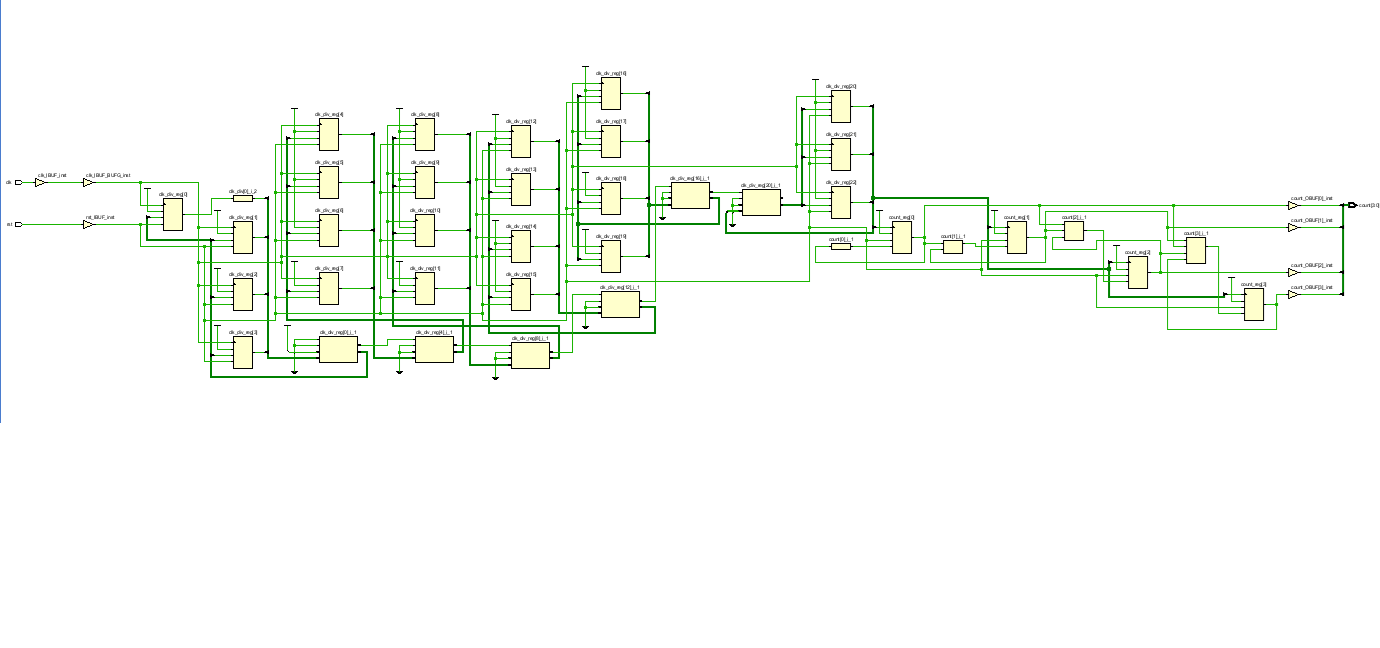
\includegraphics[width=\linewidth]{verilog_lab99.png}
\caption{Post-implementation schematic view (representative capture for the counter RTL).}
\label{fig:impl_schematic}
\end{figure}

\subsection{(5 pts) LUTs \texttt{count[0]\_i\_1}, \texttt{count[1]\_i\_1}, \texttt{count[2]\_i\_1}}

After zooming in the implemented schematic, open each cell and inspect \textbf{Cell
Properties} $\rightarrow$ \textbf{Truth Table} as instructed.

\textbf{Typical behavior for a binary up-counter (why it makes sense).}
\begin{itemize}
  \item \textbf{\texttt{count[0]\_i\_1}:}  The least significant bit toggles every active edge
        of \texttt{slow\_clk} when not held in reset.  The next-state logic for bit~0 is
        therefore equivalent to inversion (XOR with~1) of the current \texttt{count[0]} when
        enabled.  Vivado often maps this to a very small LUT (sometimes appearing like a
        1-input or 2-input slice) feeding the D-input of the register for \texttt{count[0]}.
  \item \textbf{\texttt{count[1]\_i\_1}:}  Bit~1 changes when \texttt{count[0]} carried (i.e.\
        on the cycle where \texttt{count[0]} transitions 1$\to$0), so the LUT implements
        \texttt{count[1] $\oplus$ count[0]} (half-chain of a ripple increment) or an
        equivalent minimized form with the same truth table.
  \item \textbf{\texttt{count[2]\_i\_1}:}  Similarly encodes the increment rule for
        \texttt{count[2]} based on \texttt{count[1]} and \texttt{count[0]} (carry into bit~2),
        i.e.\ XOR of \texttt{count[2]} with the AND of lower bits or the optimized equivalent.
\end{itemize}

\textbf{Does this make sense?}  \textbf{Yes.}  A synchronous binary counter is built from
flip-flops plus combinational ``next count'' logic.  Each output bit's next value is a Boolean
function of the present state (and reset); the tool packs those functions into LUTs.  The
truth tables you read in Vivado should match the minimized functions for an incrementer at
those bit positions.  \emph{Replace this paragraph with the exact truth tables and one-line
Boolean labels from your own screenshot if they differ slightly after optimization.}

% ─────────────────────────────────────────────
\section{Design Summary (reference)}

\noindent\textbf{Target device:} \texttt{xc7s25csga225-1}\\
\textbf{Ports:} \texttt{clk} (12\,MHz, pin M9), \texttt{rst} (pushbutton, pin D2),
\texttt{count[3:0]} to LEDs E2, K1, J1, E1 (LVCMOS33).\\
\textbf{Clocking:} 23-bit divider \texttt{clk\_div}; \texttt{slow\_clk = clk\_div[22]} gives
approximately $12\,\text{MHz}/2^{23} \approx 1.43$\,Hz slow updates so LED changes are visible.

\end{document}
